
\documentclass[11pt]{article} 

\usepackage{geometry} 
\geometry{a4paper} 

\usepackage{graphicx}


\title{Studio di un modello predittivo del periodo di oscillazione di un pendolo fisico}
\author{Francesco Angelo Fabiano Antonacci\\Alessandro Di Meglio}
\date{\today} 
\begin{document}
\maketitle

\section{Scopo dell'esperienza}

In questa relazione di laboratorio si intende verificare sperimentalmente il modello predittivo del periodo di un pendolo fisico dato dall'equazione (5).

\section{Cenni teorici}

Un corpo rigido sospeso in un punto diverso dal centro di massa e sottoposto all' accelerazione di gravità costituisce un pendolo fisico.
Se spostato di un angolo $\theta$ dalla posizione di equilibrio, il momento torcente agente sull corpo rispetto a al centro in cui è incernierato :
\begin{equation}
\tau  = -mgd sin(\theta)
\end{equation}

Per la seconda equazione cardinale si ha anche che:


\begin{equation}
\tau  =\frac{dL}{dt}
\end{equation}

Essendoci anche note le relazioni $L=I\omega  $ e $\omega=\frac{d\theta}{dt}$, ci è possibile ottenere la seguente equazione:

\begin{equation}
\tau=I\frac{d\theta^2}{dt^2}
\end{equation}
Combianando la (1) e la (3) otteniamo:
\begin{equation}
I\frac{d\theta^2}{dt^2}+\frac{mgd}{I}sin(\theta)=0
\end{equation}
Quest'equazione differenziale, con le dovute considerazioni discusse nella sezione "\textbf {Approssimazioni}" , è approssimabile con quella del moto armonico con $T_0=2\pi\sqrt{\frac{I}{mgd}}$ .
Con le dovute considerazioni discusse nella sezione "\textbf {Approssimazioni}", consideremo il momento di inerzia del corpo rispetto all'asse perpendicolare all'asse dell'asta passante per il centro di massa come $I_cm=\frac{ml^2}{12}$.
Per il teorema di Huygens-Steiner I in un generico asse parallelo a quello appena considerato sarà $I=\frac{ml^2}{12}+d^2m$.
Da cui otteniamo, ponendola a sistema con le precedenti, l'equazione che costituisce il modello predittivo del periodo che si intende verificare:

\begin{equation}
T(d)=2\pi\sqrt{\frac{\frac{l^2}{12}+d^2}{gd}}
\end{equation}

\section{Apparato sperimentale}
\subsection{Asta Forata}
L'oggetto che costituisce il pendolo fisico in questo esperimento è un'asta di allumino.
Lungo  una delle due sezioni più piccole passano fori identici  tra loro.

Le seguenti misure sono state prese col metro a nastro, eccetto quella dei diametri dei fori la quale è  stata effettata con il calibro ventesimale.

\begin{table}
\centering

\caption{Misure dell'asta}
\begin{tabular}[t]{|c|c|c|}
 Lunghezza asta &Spessore1&Spessore2\\
  \hline
  $1.050 \pm 0.001$ m & $0.015 \pm 0.001$ m & $0.015 \pm 0.001$ m \\
\end{tabular}

\end{table}


\begin{table}
    \centering
\caption{Diametro dei fori e rispettiva distanza dei centri da un estremo dell'asta}
    \label{tab:lunghezza-asta}
    \begin{tabular}{|c|c|}
        \hline
        Diametro & Distanza\\
        \hline
         $0.005 \pm 0.0005$ m & $0.050 \pm 0.001$ m \\
        $0.005 \pm 0.0005$ & $0.150 \pm 0.001$ m \\
        $0.005 \pm 0.0005$ & $0.250\pm 0.001$ m \\
        $0.005 \pm 0.0005$ & $0.350 \pm 0.001$ m \\
        $0.005 \pm 0.0005$ & $0.450 \pm 0.001$ m \\
        $0.005 \pm 0.0005$  & $0.550 \pm 0.001$ m \\
        $0.005 \pm 0.0005$ & $0.650 \pm 0.001$ m \\
       $0.005 \pm 0.0005$ & $0.750 \pm 0.001$ m \\
       $0.005 \pm 0.0005$ & $0.850 \pm 0.001$ m \\
        $0.005 \pm 0.0005$ & $0.950 \pm 0.001$ m \\
        \hline
    \end{tabular}
\end{table}

\subsection{Supporto}
L'asta è stata incernierata alla parte terminale di un supporto, consistente in una barra metellica disposta parallela al terreno. 
Il vincolo della cerniera era una vite passante per i fori dell'asta e poggiante su cuscinetti a sfera per ridurre l'attrito durante il movimento.
Leggere la sezione "\textbf{Approssimazioni}" in merito al comportamento del supporto durante l'esperimento.


\subsection{Strumenti di misura}
\begin{enumerate}
\item Cronometro digitale con risoluzione di un centesimo di secondo.
\item Metro a nastro con risoluzione di un millimetro.
\item Calibro con risoluzione di un ventesimo di millimetro.

\end{enumerate}
\section{Descrizione delle misure}

\begin{table}
    \centering
    \caption{Misure di 5 periodi iterate 10 volte per ciascuno dei 10 fori }
 
    \begin{tabular}{|c|c|c|c|c|c|c|c|c|c|}
        \hline
        \textbf{F1} & \textbf{F2} & \textbf{F3} & \textbf{F4} & \textbf{F5} & \textbf{F6} & \textbf{F7} & \textbf{F8} & \textbf{F9} & \textbf{F10} \\
        \hline
 
  8.04 & 7.85 & 7.80 & 8.37 & 11.40 & 19.01 & 9.29 & 7.99 & 7.80 & 7.94 \\
  8.35 & 7.89 & 7.85 & 8.44 & 11.29 & 18.91 & 9.29 & 8.09 & 7.91 & 7.98 \\
  8.04 & 7.92 & 7.80 & 8.37 & 11.35 & 18.76 & 9.24 & 8.01 & 7.86 & 8.04 \\
  8.19 & 7.84 & 7.77 & 8.42 & 11.40 & 18.97 & 9.50 & 8.05 & 7.77 & 8.06 \\
  8.13 & 7.91 & 7.86 & 8.32 & 11.54 & 19.00 & 9.35 & 7.97 & 7.79 & 8.17 \\
  8.13 & 7.78 & 7.92 & 8.38 & 11.35 & 19.04 & 9.30 & 8.04 & 7.83 & 7.92 \\
  8.13 & 7.85 & 7.76 & 8.22 & 11.41 & 18.84 & 9.36 & 7.99 & 7.87 & 7.96 \\
  8.18 & 7.96 & 7.79 & 8.30 & 11.48 & 18.85 & 9.31 & 8.04 & 7.86 & 7.91 \\
  8.16 & 7.99 & 7.84 & 8.31 & 11.40 & 18.92 & 9.37 & 7.98 & 7.83 & 8.10 \\
  8.17 & 7.99 & 7.86 & 8.26 & 11.39 & 18.66 & 9.29 & 8.03 & 7.90 & 8.11 \\
 \hline
    \end{tabular}
\end{table}


\subsection{Approssimazioni}
\subsubsection{Supporto}
E' stato osservato che nonostante il supporto del particolare esperimento fosse potenzialmente soggetto ad oscillazioni in tutti i gradi di libertà per effetti di elasticità, nelle particolari sollecitazioni dell'esperimento è ragionevole supporlo come immobile in quanto gli effetti non sono osservabili dall'occhio umano.
\subsubsection{Momento di inerzia}
Supposto momentanamente che l'asta fosse omogenea, il momento di inerzia dell'asta considerata come un parallelepipedo omogeneo è $I=\frac{(l^2+s^2)m}{12}$.
Ma $\sigma_b ^2 \ll \sigma_a 2a$ di un ordine di grandezza, pertanto un effetto della larghezza della sbarra nella variazione del momento di inerzia e ,pertanto, del periodo non sarebbe apprezzabile per l'effetto che già ha l'errore di misura della lunghezza dell'asta.
\subsubsection{Piccole Oscillazioni}
Per poter ridurre l'approssimazione del seno al primo temine della serie al fine di semplificare l'equazione differenziale (5), deve essere soddisfatta la seguente condizione: $\theta_0 \ll 4\sqrt{\frac{\sigma T}{T}}$, ovvero l'errore relativo della misura del tempo deve essere molto maggiore del secondo termine dello sviluppo della serie (gli altri termini continuano a soddisfare la relazione in quanto sono ciascuno diversi ordini di grandezza inferiori al precedente).

\section{Analisi dei dati}
\begin{figure}[htbp]
\centerline{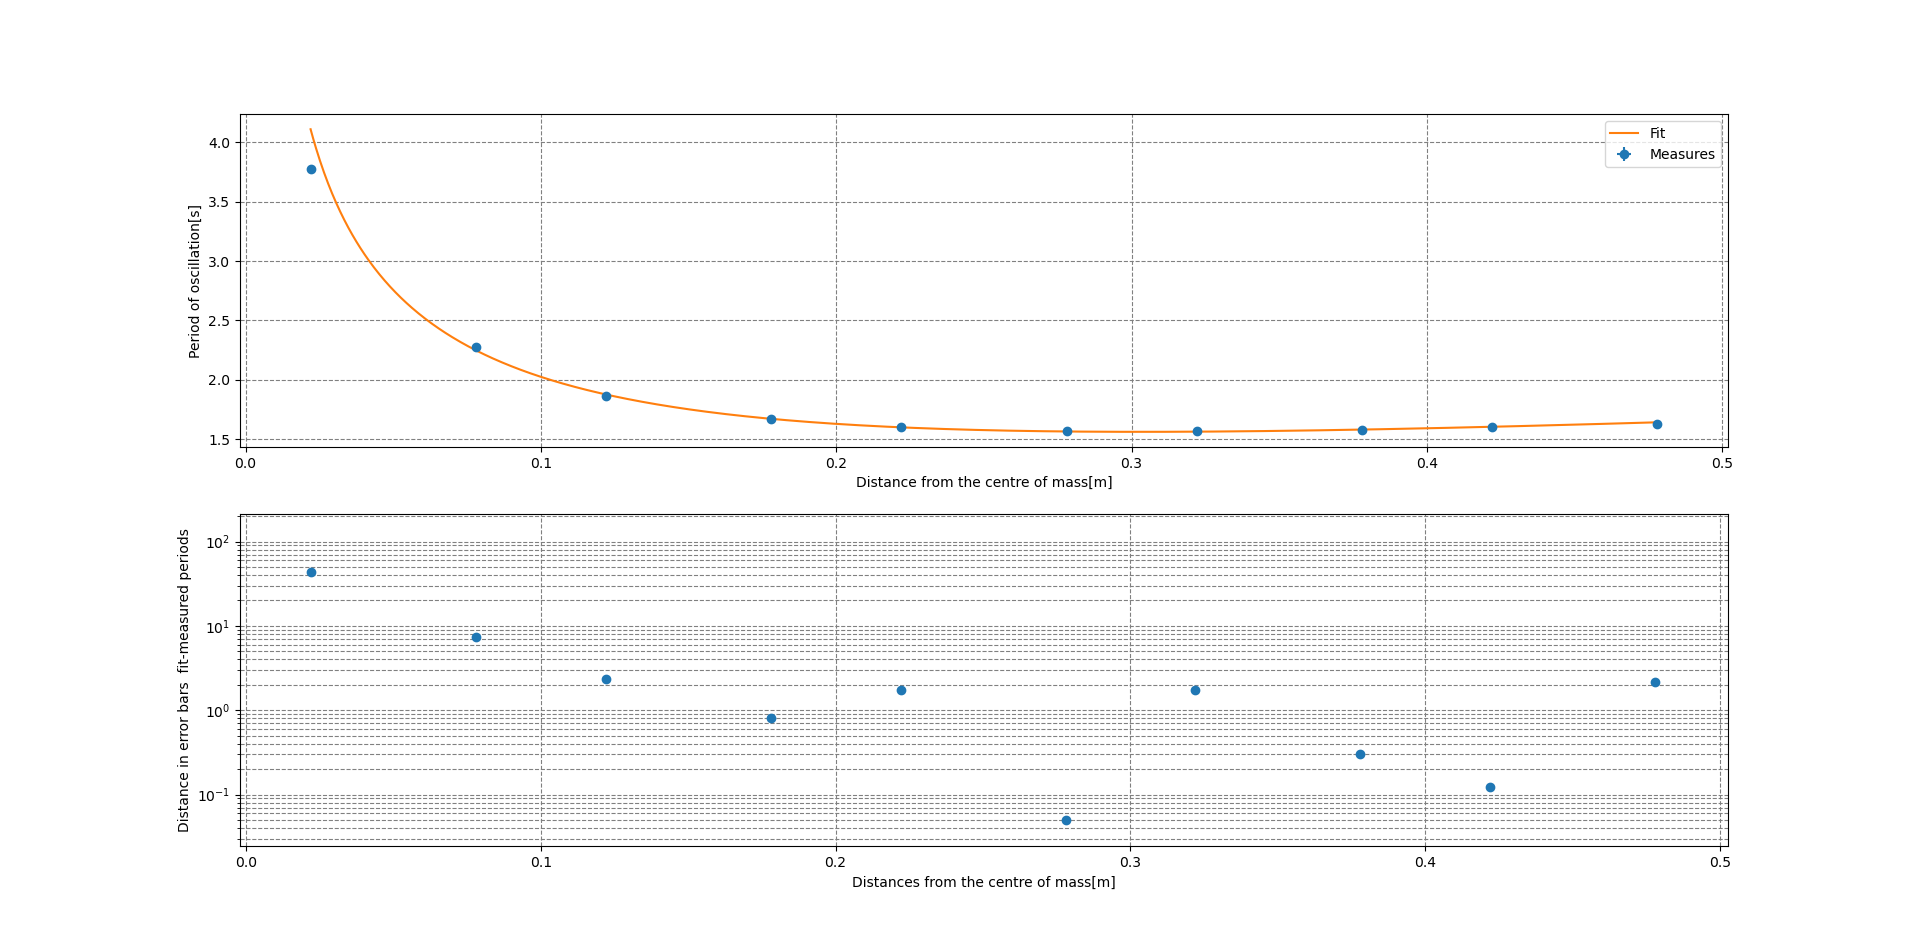
\includegraphics[width=20cm, height=15cm]{physicalpendulum_plots_1.0.png}}

\label{fig}
\end{figure}

\section{Conclusione}

\end{document}
